%%%%%%%%%%%%%%%%%%%%%%%%%%%%%%%%%%%%%%%%%
% Programming/Coding Assignment
% LaTeX Template
%
% This template has been downloaded from:
% http://www.latextemplates.com
%
% Original author:
% Ted Pavlic (http://www.tedpavlic.com)
%
% Note:
% The \lipsum[#] commands throughout this template generate dummy text
% to fill the template out. These commands should all be removed when 
% writing assignment content.
%
% This template uses a Perl script as an example snippet of code, most other
% languages are also usable. Configure them in the "CODE INCLUSION 
% CONFIGURATION" section.
%
%%%%%%%%%%%%%%%%%%%%%%%%%%%%%%%%%%%%%%%%%

%----------------------------------------------------------------------------------------
%	PACKAGES AND OTHER DOCUMENT CONFIGURATIONS
%----------------------------------------------------------------------------------------

\documentclass{article}

\usepackage{fancyhdr} % Required for custom headers
\usepackage{lastpage} % Required to determine the last page for the footer
\usepackage{extramarks} % Required for headers and footers
\usepackage[usenames,dvipsnames]{color} % Required for custom colors
\usepackage{graphicx} % Required to insert images
\usepackage{listings} % Required for insertion of code
\usepackage{courier} % Required for the courier font
\usepackage{lipsum} % Used for inserting dummy 'Lorem ipsum' text into the template

\usepackage{enumerate}
\usepackage{amsmath}
\usepackage{hyperref}

\usepackage{graphicx}
\usepackage{caption}
\usepackage{subcaption}

\usepackage{listings}
\usepackage{color} %red, green, blue, yellow, cyan, magenta, black, white
\usepackage{gensymb}

\definecolor{mygreen}{RGB}{28,172,0} % color values Red, Green, Blue
\definecolor{mylilas}{RGB}{170,55,241}

% Margins
\topmargin=-0.45in
\evensidemargin=0in
\oddsidemargin=0in
\textwidth=6.5in
\textheight=9.0in
\headsep=0.25in

\linespread{1.1} % Line spacing

% Set up the header and footer
\pagestyle{fancy}
\lhead{\hmwkAuthorName} % Top left header
\chead{\hmwkClass\ (\hmwkClassInstructor\ \hmwkClassTime): \hmwkTitle} % Top center head
\rhead{\firstxmark} % Top right header
\lfoot{\lastxmark} % Bottom left footer
\cfoot{} % Bottom center footer
\rfoot{Page\ \thepage\ of\ \protect\pageref{LastPage}} % Bottom right footer
\renewcommand\headrulewidth{0.4pt} % Size of the header rule
\renewcommand\footrulewidth{0.4pt} % Size of the footer rule

\setlength\parindent{0pt} % Removes all indentation from paragraphs

%----------------------------------------------------------------------------------------
%	CODE INCLUSION CONFIGURATION
%----------------------------------------------------------------------------------------

\definecolor{MyDarkGreen}{rgb}{0.0,0.4,0.0} % This is the color used for comments
\lstloadlanguages{Perl} % Load Perl syntax for listings, for a list of other languages supported see: ftp://ftp.tex.ac.uk/tex-archive/macros/latex/contrib/listings/listings.pdf
\lstset{language=Perl, % Use Perl in this example
        frame=single, % Single frame around code
        basicstyle=\small\ttfamily, % Use small true type font
        keywordstyle=[1]\color{Blue}\bf, % Perl functions bold and blue
        keywordstyle=[2]\color{Purple}, % Perl function arguments purple
        keywordstyle=[3]\color{Blue}\underbar, % Custom functions underlined and blue
        identifierstyle=, % Nothing special about identifiers                                         
        commentstyle=\usefont{T1}{pcr}{m}{sl}\color{MyDarkGreen}\small, % Comments small dark green courier font
        stringstyle=\color{Purple}, % Strings are purple
        showstringspaces=false, % Don't put marks in string spaces
        tabsize=5, % 5 spaces per tab
        %
        % Put standard Perl functions not included in the default language here
        morekeywords={rand},
        %
        % Put Perl function parameters here
        morekeywords=[2]{on, off, interp},
        %
        % Put user defined functions here
        morekeywords=[3]{test},
       	%
        morecomment=[l][\color{Blue}]{...}, % Line continuation (...) like blue comment
        numbers=left, % Line numbers on left
        firstnumber=1, % Line numbers start with line 1
        numberstyle=\tiny\color{Blue}, % Line numbers are blue and small
        stepnumber=5 % Line numbers go in steps of 5
}

% Creates a new command to include a perl script, the first parameter is the filename of the script (without .pl), the second parameter is the caption
\newcommand{\perlscript}[2]{
\begin{itemize}
\item[]\lstinputlisting[caption=#2,label=#1]{#1.pl}
\end{itemize}
}

%----------------------------------------------------------------------------------------
%	DOCUMENT STRUCTURE COMMANDS
%	Skip this unless you know what you're doing
%----------------------------------------------------------------------------------------

% Header and footer for when a page split occurs within a problem environment
\newcommand{\enterProblemHeader}[1]{
\nobreak\extramarks{#1}{#1 continued on next page\ldots}\nobreak
\nobreak\extramarks{#1 (continued)}{#1 continued on next page\ldots}\nobreak
}

% Header and footer for when a page split occurs between problem environments
\newcommand{\exitProblemHeader}[1]{
\nobreak\extramarks{#1 (continued)}{#1 continued on next page\ldots}\nobreak
\nobreak\extramarks{#1}{}\nobreak
}

\setcounter{secnumdepth}{0} % Removes default section numbers
\newcounter{homeworkProblemCounter} % Creates a counter to keep track of the number of problems

\newcommand{\homeworkProblemName}{}
\newenvironment{homeworkProblem}[1][Problem \arabic{homeworkProblemCounter}]{ % Makes a new environment called homeworkProblem which takes 1 argument (custom name) but the default is "Problem #"
\stepcounter{homeworkProblemCounter} % Increase counter for number of problems
\renewcommand{\homeworkProblemName}{#1} % Assign \homeworkProblemName the name of the problem
\section{\homeworkProblemName} % Make a section in the document with the custom problem count
\enterProblemHeader{\homeworkProblemName} % Header and footer within the environment
}{
\exitProblemHeader{\homeworkProblemName} % Header and footer after the environment
}

\newcommand{\problemAnswer}[1]{ % Defines the problem answer command with the content as the only argument
\noindent\framebox[\columnwidth][c]{\begin{minipage}{0.98\columnwidth}#1\end{minipage}} % Makes the box around the problem answer and puts the content inside
}

\newcommand{\homeworkSectionName}{}
\newenvironment{homeworkSection}[1]{ % New environment for sections within homework problems, takes 1 argument - the name of the section
\renewcommand{\homeworkSectionName}{#1} % Assign \homeworkSectionName to the name of the section from the environment argument
\subsection{\homeworkSectionName} % Make a subsection with the custom name of the subsection
\enterProblemHeader{\homeworkProblemName\ [\homeworkSectionName]} % Header and footer within the environment
}{
\enterProblemHeader{\homeworkProblemName} % Header and footer after the environment
}

%----------------------------------------------------------------------------------------
%	NAME AND CLASS SECTION
%----------------------------------------------------------------------------------------

\newcommand{\hmwkTitle}{Homework\ \#6} % Assignment title
\newcommand{\hmwkDueDate}{Thursday,\ October\ 22,\ 2015} % Due date
\newcommand{\hmwkClass}{CSC 514: Computer Vision} % Course/class
\newcommand{\hmwkClassTime}{11:00am} % Class/lecture time
\newcommand{\hmwkClassInstructor}{Hoover} % Teacher/lecturer
\newcommand{\hmwkAuthorName}{Julian A. Brackins} % Your name

%----------------------------------------------------------------------------------------
%	TITLE PAGE
%----------------------------------------------------------------------------------------

\title{
\vspace{2in}
\textmd{\textbf{\hmwkClass:\ \hmwkTitle}}\\
\normalsize\vspace{0.1in}\small{Due\ on\ \hmwkDueDate}\\
\vspace{0.1in}\large{\textit{\hmwkClassInstructor\ \hmwkClassTime}}
\vspace{3in}
}

\author{\textbf{\hmwkAuthorName}}
\date{} % Insert date here if you want it to appear below your name

%----------------------------------------------------------------------------------------

\begin{document}

\maketitle

%----------------------------------------------------------------------------------------
%	TABLE OF CONTENTS
%----------------------------------------------------------------------------------------

%\setcounter{tocdepth}{1} % Uncomment this line if you don't want subsections listed in the ToC

\newpage

\newpage

%----------------------------------------------------------------------------------------
%	PROBLEM 1
%----------------------------------------------------------------------------------------

% To have just one problem per page, simply put a \clearpage after each problem

\begin{homeworkProblem}
In class we discussed several different methods for performing filtering/template matching on images. In this homework you will create your own Matlab functions to perform both convolution and correlation on images using different convolution/correlation kernels.

\section{Preface}
Before we can answer \textit{Where's Waldo}, we must first ask the question, \textit{Who} is Waldo? \\
\textit{Where's Wally?}, also known as \textit{Where's Waldo} in the United States and Canada, is a children's book series created by English Illustrator Martin Handford. The books consist of double-paged illustrations containing hundreds of persons in a given location. In each scene, Waldo is hidden amongst the group, wearing his signature red and white striped shirt, bobble hat, and spectacles. \textit{(source: Wikipedia)}

This assignment involves automating the process of finding Waldo in a Where's Waldo scene. This will be done using correlation to match features in two different images.

\section{Equations}
The two equations being used for this assignment are the Correlation and Convolution equations. \\ \\
\textbf{Correlation:} $$G\Big[ i , j \Big] = \sum\limits_{u=-k}^{k} \sum\limits_{v=-k}^{k} H\Big[ u , v \Big]F\Big[ i + u , j + v \Big]$$ \\

Where $F$ is the image and $H$ is the kernel. \\
This is referred to as cross-correlation. In Image filtering, convolution is performed by replacing each pixel with a linear combination of its neighbors. Then, the \textit{filter} (interchangeably referred to as a \textit{kernel} or \textit{mask} henceforth) is used to describe the weights in the linear combination. For any given pixel in the image, the greater the intensity value after this correlation filter is applied, the closer that pixel is in relation to the kernel image. Figure~\ref{fig:surf} details the intensity map generated from performing cross correlation on the Waldo Scene and Waldo Kernel.

\textbf{Convolution:} $$G\Big[ i , j \Big] = \sum\limits_{u=-k}^{k} \sum\limits_{v=-k}^{k} H\Big[ u , v \Big]F\Big[ i - u , j - v \Big]$$ \\

Where $F$ is the image and $H$ is the kernel. \\ 
Convolution can actually be performed using Correlation. Flip the kernel in both directions (or rotate the kernel 180\degree), then apply correlation.

\section{Process}

The following is the process used to find Waldo.
\begin{itemize}
	\item Read in the Kernel and Scene Images
	
	\begin{figure}
\centering
\begin{subfigure}{.5\textwidth}
  \centering
  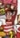
\includegraphics[width=.05\linewidth]{img/WaldoKernel}
  \caption{Image Kernel}
  \label{fig:sub1}
\end{subfigure}%
\begin{subfigure}{.5\textwidth}
  \centering
  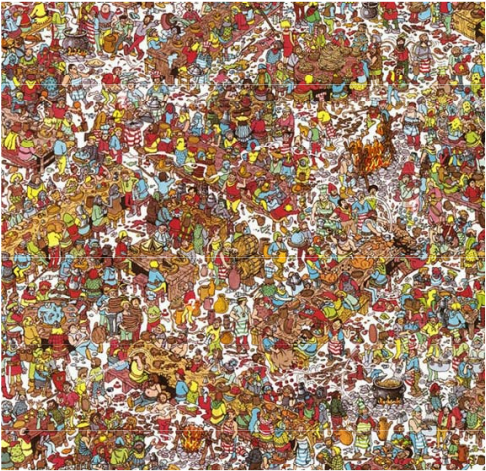
\includegraphics[width=.95\linewidth]{img/WaldoScene}
  \caption{Waldo Scene}
  \label{fig:sub2}
\end{subfigure}
\caption{Waldo Images}
\label{fig:waldo}
\end{figure}	
	
	\item Convert Kernel and Scene to Grayscale
	\item Find Dimensions of the Scene and Kernel
	\item Divide Kernel in Half so that we work with a smaller kernel size.
	\item Calculate Correlation or Convolution.
	\item Find Waldo by locating the highest value point in the $G$ Matrix.
	\item Display Original Scene with Kernel superimposed on Waldo's location.

\end{itemize}

\subsection{Correlation}
The following pseudocode is the process for calculating Correlation:

\begin{itemize}
	\item Find the dimensions for the scene and kernel
	\item Set H = kernel, F = scene, G = result so that program matches formulas above
	\item Divide Kernel so that we work with a smaller kernel size.
	\item Generate Mean for Scene and Kernel
	\item Perform Correlation by applying the weighted kernel value to each pixel in the image.
\end{itemize}

The resultant $G$ Matrix generated by the correlation function yields the 3D surface mapping found in Figure~\ref{fig:surf}.


\begin{figure}
\centering
\begin{subfigure}{.5\textwidth}
  \centering
  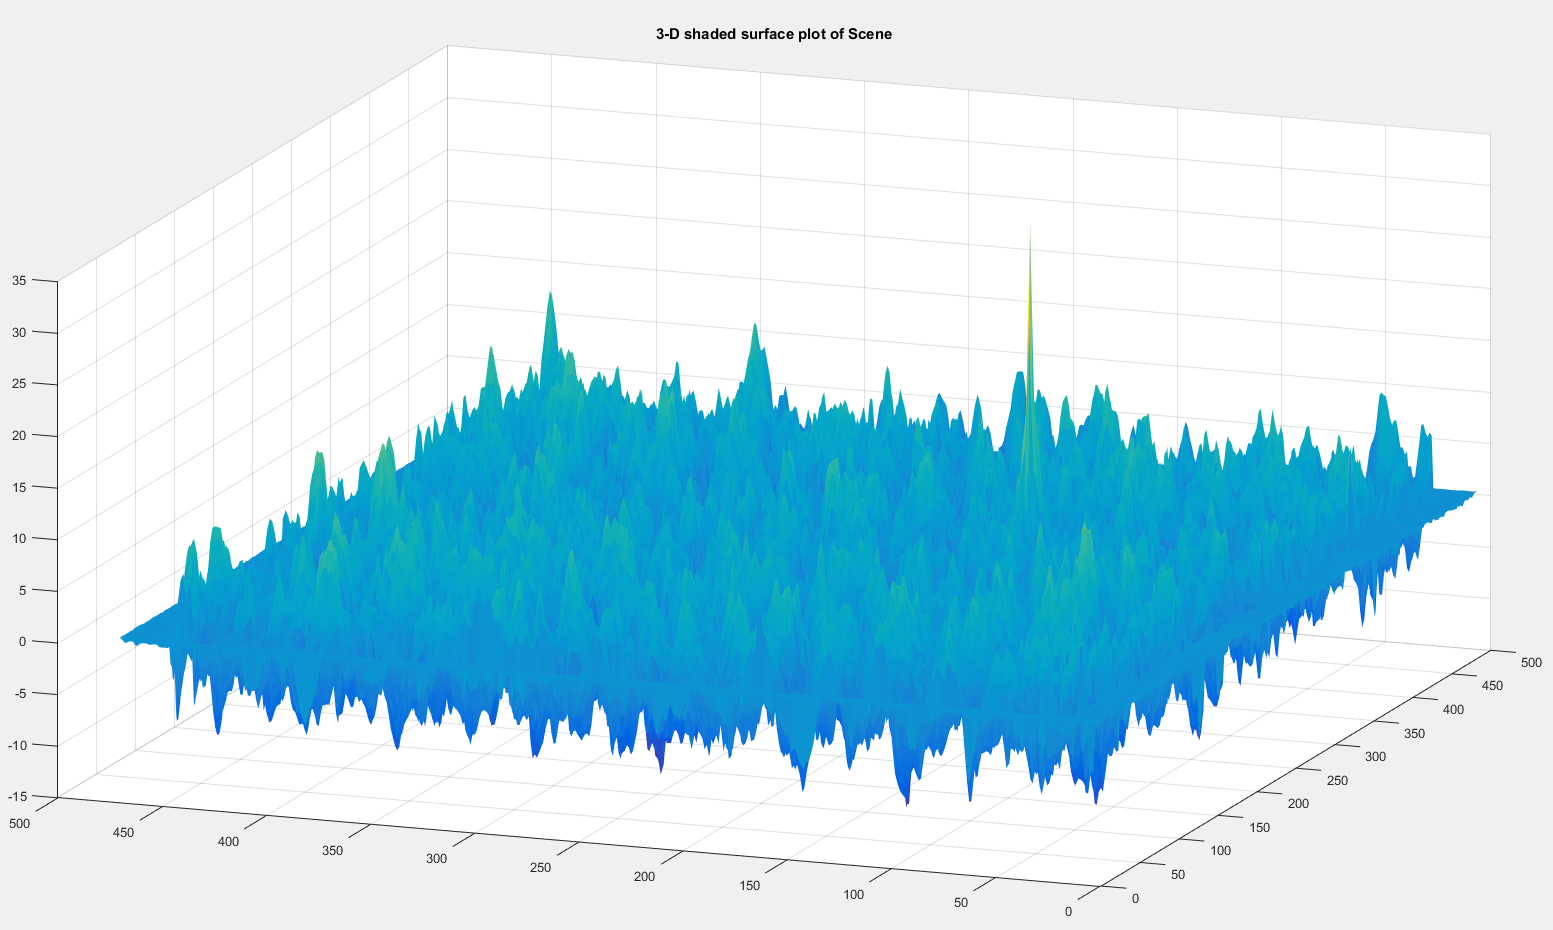
\includegraphics[width=.9\linewidth]{img/surf1}
  \caption{3D Surface Graph.}
  \label{fig:sub1}
\end{subfigure}%
\begin{subfigure}{.5\textwidth}
  \centering
  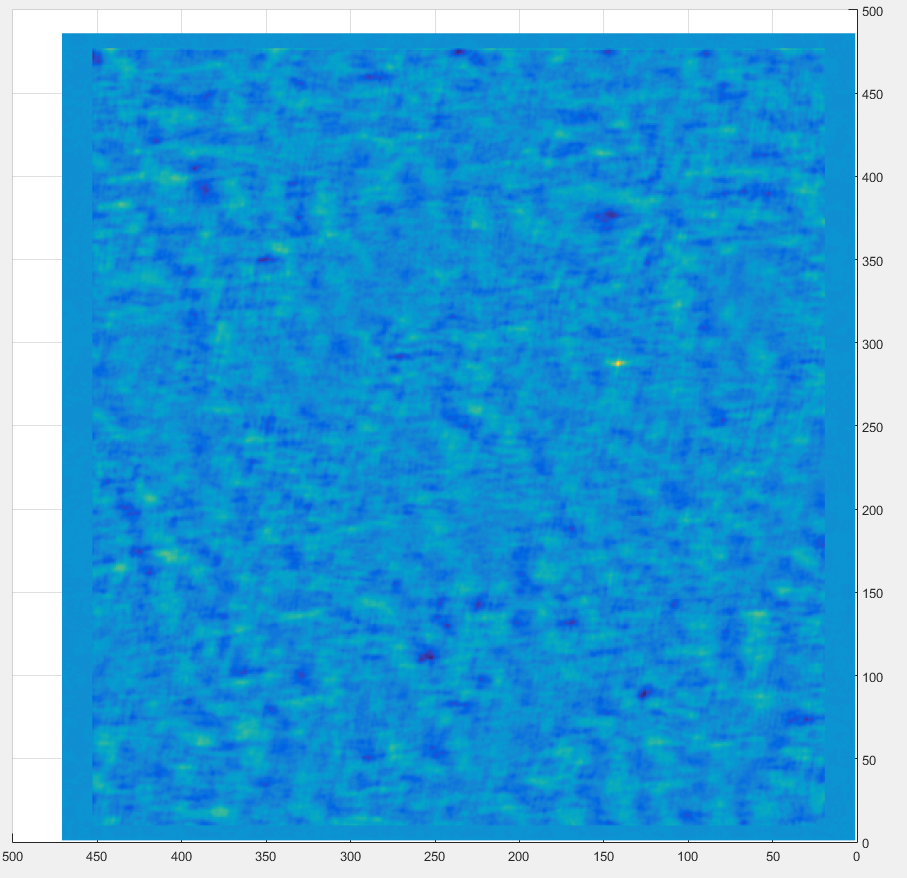
\includegraphics[width=.9\linewidth]{img/surf2}
  \caption{Top-Down View.}
  \label{fig:sub2}
\end{subfigure}
\caption{3D surface of image after applying correlation}
\label{fig:surf}
\end{figure}

The image displayed in Figure~\ref{fig:subguess} is the scene after the correlation filter is applied. A noticeable peak is observed in the image, which will be used as a guess for Waldo's Location. Using the x,y coordinates of that peak, we can now superimpose the kernel onto the original image, as shown in Figure~\ref{fig:subsolve}.

\begin{figure}
\centering
\begin{subfigure}{.5\textwidth}
  \centering
  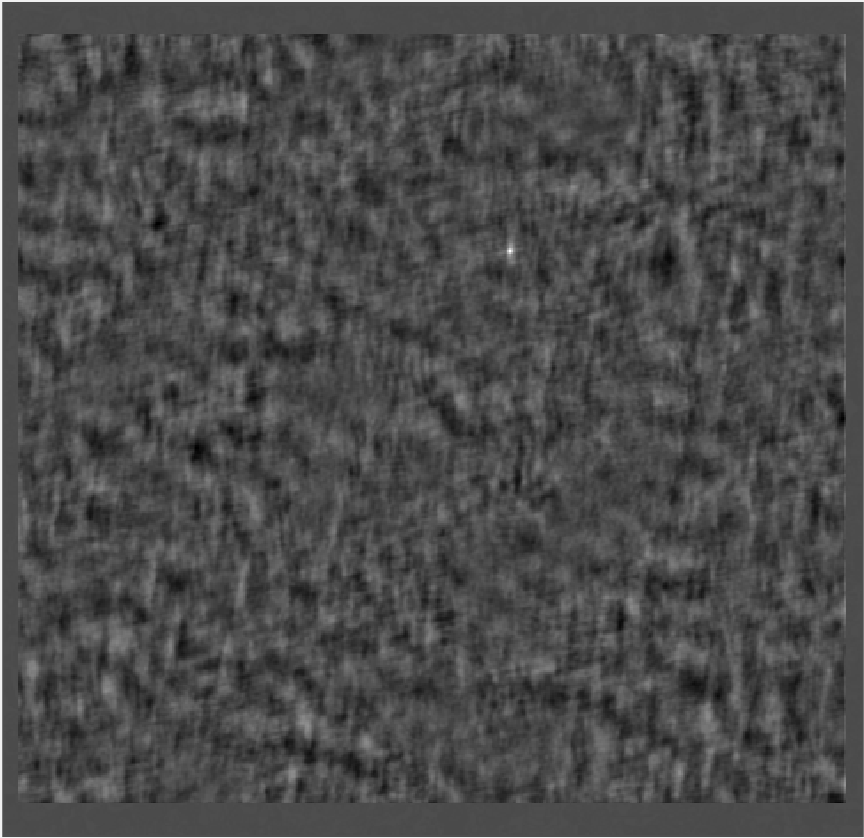
\includegraphics[width=.95\linewidth]{img/guess}
  \caption{Image after applying Correlation}
  \label{fig:subguess}
\end{subfigure}%
\begin{subfigure}{.5\textwidth}
  \centering
  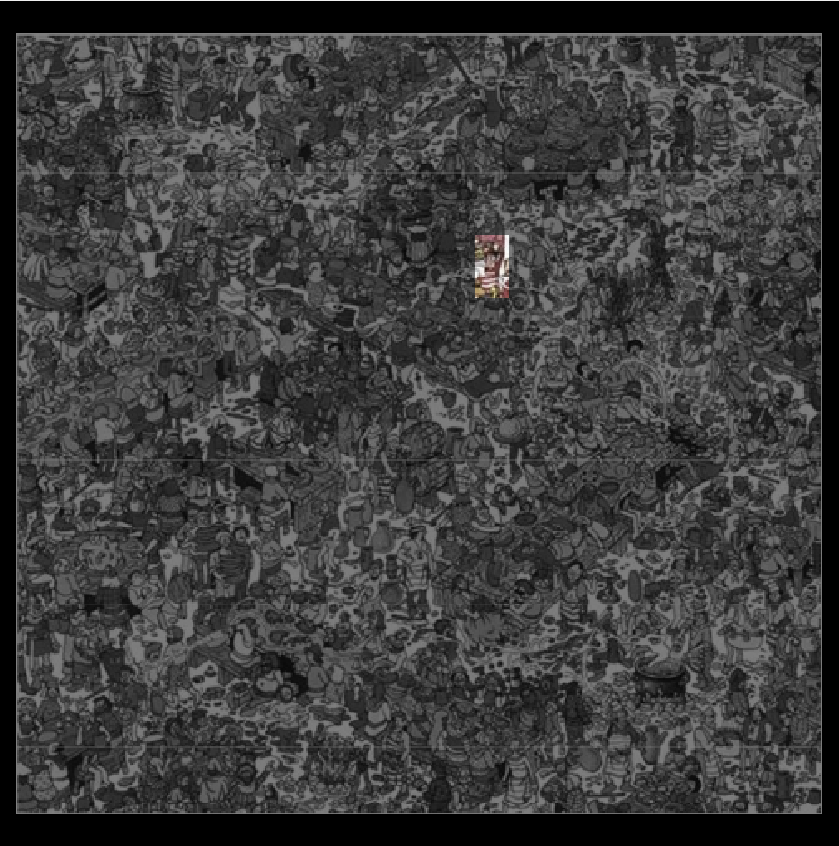
\includegraphics[width=.95\linewidth]{img/WaldoSolved}
  \caption{Kernel superimposed onto original scene.}
  \label{fig:subsolve}
\end{subfigure}
\caption{Finding Waldo}
\label{fig:soln}
\end{figure}


\subsection{Convolution}
As stated earlier, Convolution is done similarly to Correlation. However, the resultant image returned from performing Convolution (Figure~\ref{fig:bad}) did not produce the same accurate guess for Waldo's location that was observed in the Correlation equation.


\begin{figure}
\centering
\begin{subfigure}{.5\textwidth}
  \centering
  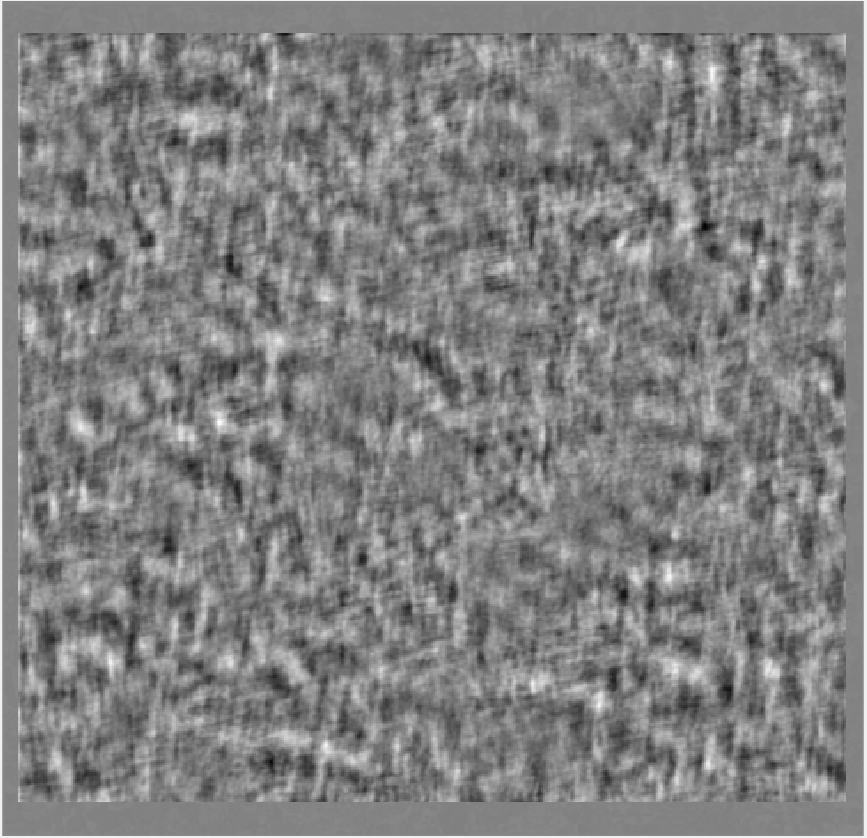
\includegraphics[width=1\linewidth]{img/guessBad}
  \caption{Image after applying Correlation}

\end{subfigure}%

\caption{Image after applying Convolution}
\label{fig:bad}
\end{figure}




\section{Matlab}
The Matlab Code for the program attached after the conclusion of this Homework Document.

\section{Conclusion}
This assignment was a study in utilizing template matching to discover similar features between two images. This was done by writing Matlab functions to perform correlation and convolution.\\
Correlation and Convolution are two different methods for filtering discussed and examined during this homework assignment. Correlation worked well as the Waldo search algorithm because the formula focuses on finding the similarities between two matrices. On the other hand, the convolution formula did not work well for finding Waldo, as convolution is more useful in discovering how two matrices differ from one another.



\lstset{language=Matlab,%
    %basicstyle=\color{red},
    breaklines=true,%
    morekeywords={matlab2tikz},
    keywordstyle=\color{blue},%
    morekeywords=[2]{1}, keywordstyle=[2]{\color{black}},
    identifierstyle=\color{black},%
    stringstyle=\color{mylilas},
    commentstyle=\color{mygreen},%
    showstringspaces=false,%without this there will be a symbol in the places where there is a space
    numbers=left,%
    numberstyle={\tiny \color{black}},% size of the numbers
    numbersep=9pt, % this defines how far the numbers are from the text
    emph=[1]{for,end,break},emphstyle=[1]\color{red}, %some words to emphasise
    %emph=[2]{word1,word2}, emphstyle=[2]{style},    
}

\clearpage
\begin{lstlisting}[caption = {Where's Waldo Script}]
function wheres_waldo()
    %%Read in Kernel, convert to grayscale double. Save original copy.
    kernel = imread('WaldoKernel.png');
    orig_kern = kernel;
    kernel = rgb2gray(kernel);
    kernel = im2double(kernel);

    %%Read in Scene, convert to grayscale double. Save original copy.
    scene = imread('WaldoScene.png');
    orig_scene = scene;
    scene = rgb2gray(scene);
    scene = im2double(scene);

    %%Find the dimensions for the scene and kernel
    [kH, kW] = size(kernel);
    [sH, sW] = size(scene);
    
     %%Divide Kernel Height and Width
    kH = kH/2;
    kW = kW/2;
    
    %%Calculate Correlation
    G =  correlation( scene, kernel );
    %%OR you can do convolution...
    %%G =  convolution( scene, kernel );
    %%Actually don't because convlution is trash for this program...

    %%Find Waldo by finding the highest value point
    [r,c] = find(G==max(G(:)));

    %%Pad array so that the imposed image lines up properly
    scene  = padarray(scene,[kH,kW]);
    orig_kern = padarray(orig_kern,[r,c],'pre');
    orig_kern = padarray(orig_kern,[sH-r,sW-c],'post');

    %%Show the Original Image
    figure, imshow(orig_scene,[]);
    title('Original Scene');

    %%Show the surf Image
    figure, surf(G), shading flat;
    title('Quantized Samples');

    %%Show the G matrix
    figure, imshow(G,[]);
    title('Waldo Guess location');

    %%Show the Search Result
    figure, imshowpair(scene(:,:,1),orig_kern,'blend');
    title('Kernel Superimposed on Original Image');

end
\end{lstlisting}

\clearpage


\begin{lstlisting}[caption = {Correlation Function}]
function [ G ] = correlation( scene, kernel )
    %%Find the dimensions for the scene and kernel
    [kH, kW] = size(kernel);
    [sH, sW] = size(scene);


    %%set F, G, H matrices so that they match what's in the book.
    G = scene;
    F = scene;
    H = kernel;

    %%Divide Kernel Height and Width so we work with a smaller kern
    kH = kH/2;
    kW = kW/2;

    %%Generate Mean for Scene and Kernel
    meanS = mean(mean(scene));
    meanK = mean(mean(kernel));


    %%Perform Correlation
    for i=(kH):(sH-kH)
        for j=(kW):(sW-kW)
            G(i,j) = sum(sum((F(i-kH+1:i+kH, j-kW+1:j+kW)-meanS).*(H-meanK)));
        end
    end
end
\end{lstlisting}

\begin{lstlisting}[caption = {Convolution Function}]
    %%For Convolution, just Flip the filter in both directions
    kernel = rot90(kernel,2);
    [kH, kW] = size(kernel);
    [sH, sW] = size(scene);

    G = scene;
    F = scene;
    H = kernel;

    kH = kH/2;
    kW = kW/2;

    meanS = mean(mean(scene));
    meanK = mean(mean(kernel));

    %%Perform Correlation
    for i=(kH):(sH-kH)
        for j=(kW):(sW-kW)
            G(i,j) = sum(sum((F(i-kH+1:i+kH, j-kW+1:j+kW)-meanS).*(H-meanK)));
        end
    end
end
\end{lstlisting}


\end{homeworkProblem}
\clearpage

%----------------------------------------------------------------------------------------

\end{document}